\prefacesection{Justification/Benefits}

\section*{Popularity}
The field of neural network machine learning algorithms have become subsequently popular in recent years, 
especially in the subset of convolutional neural network (CNN's). Figure 1 below displays the Google trends
graphs of the search term "Convolutional Neural Network". As seen in the graph, the scale from 0 to 100
represents the least to the highest level of interest from 2004 to the present year. 
A upsurge occurs approximately around January of 2016 \citep{trends}.

\begin{figure}[ht]
\begin{center}
    \advance\leftskip-3cm
    \advance\rightskip-3cm
    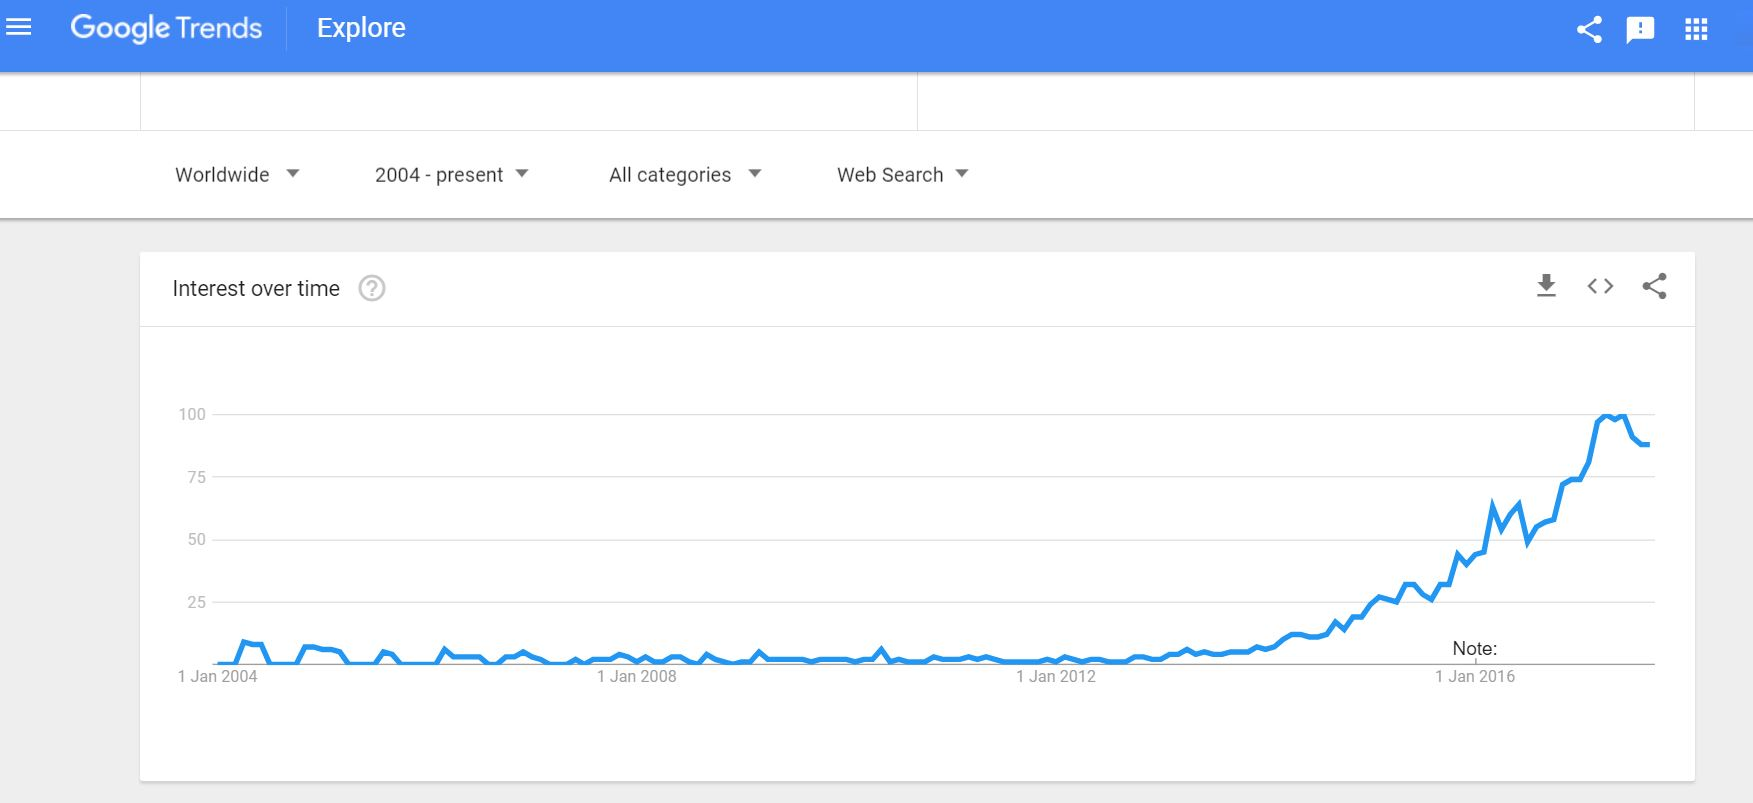
\includegraphics[keepaspectratio=true,scale=0.6]{resources/cnn-trends.jpg}
    \caption{Google Trends Graph of Search Queries for CNN's}
    \label{pop}
\end{center}
\end{figure}


\subsubsection*{Social Media}
The researcher and founded of convolutional neural networks (CNN's), Yann LeCun, became the director of Facebook's Artificial Intelligence department in 2013, and it is said believed that Facebook uses CNN's for it's facial recognition, user classification and tagging features \citep{adit}. CNN's, in conjunction with recurrent nets, are also used for Facebooks DeepText feature. DeepText is a deep learning text-understanding engine used to comprehend and classify human generated textual content in over 20 languages \citep{DeepText}.

\subsection*{Medicine}
In recent year, neural network have been used in the field of medicine to better predict diagnoses and detection of cancerous tumours. For example, CNN's have been used by researchers for brain tumor segmentation \citep{DBLP}. Havaei et al state in their research that difficulties may arise when utilising regular magnetic resonance imaging (MRI) to segment glioblastomas (GBM) tumours from the rest of the brain as may appear in different areas and sizes. CNN's were trained and have learned to better approach the problem with segmentation. The use of CNN's proved appropriate methods for tumour segmentation as the results can be given from a range of 25 seconds to 3 minutes \citep{DBLP}. \\
Furthermore, artificial neural networks have been used by radiologists for Computer-Aided detections systems (CADe) and Computer-aided Diagnosis systems (CADx) to improve the accuracy of diagnoses, early detections and to minimize the time spent on evaluation by doctors \citep{CADe}. Although the use of these computational systems prove to be advantageous, \citeauthor{CADe} state that further work is needed to better improve the practicality of these detection methodologies. Some of the challenges and improvements needed, to name a few, are integration of CADe and CADx systems to a hospital environments, further work on reducing the number of false positive results and larger databases to be provided for a more accurate prognosis. 

\section*{Business}
Many businesses depend on artificial neural networks for their business model.
Artificial neural networks can be applied to many industries and disciplines. According to \citet{geocities}
artificial neural networks are used in the following range of business applications:
\subsubsection*{Marketing}
\begin{itemize}
	\item Forecasting of sales
	\item Classification of spending patterns 
	\item market targeting
\end{itemize}

\subsubsection*{Finance}
\begin{itemize}
	\item Risk Analysis
	\item Financial Forecasting - The estimation of future revenue expenditures trends.
	\item Bankruptcy prediction. 
\end{itemize}

\subsection*{Workplace Productivity}
Neural networks have been used for emotion detection within organizations to boost productivity. According to studies, emotions have strong influence on a competitive marketplace. These factors are intellectual capital, customer service, organizational reactivity, production, appeal of the employee and retentivity \citep{empdetect}. \citeauthor{empdetect} suggest in their proposal that facial detection software could be used by organizations to better observe the overall emotions of their employees and to prevent negative sentiment to affect company productivity.

